\frame{
\frametitle{Arquitectura de Von Neumann}
\begin{columns}
\begin{column}{0.59\textwidth}
\begin{itemize}
\item Fue publicada por primera vez por John von Neumann en 1945.
\item Su diseño de arquitectura informática consta de una Unidad de Control, Unidad Aritmética y Lógica (ALU), Unidad de Memoria, Registros y Entradas / Salidas.
\item La arquitectura de Von Neumann se basa en el concepto de computadora de programa almacenado, donde los datos de instrucción y los datos del programa se almacenan en la misma memoria. 
\end{itemize}
\end{column}
\begin{column}{0.39\textwidth}
\begin{center}
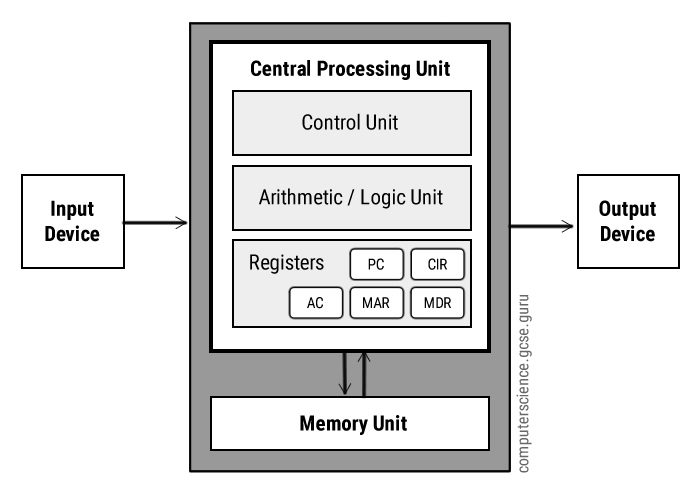
\includegraphics[width=0.9\textwidth]{Figs/Von-Neumann-Architecture-Diagram}\\
\end{center}
\begin{block}{Secuencia de operaciones}
\textbf{En serie.}
\end{block}
\end{column}
\end{columns}
}



%\subsection{FPGAs y sus componentes b\'asicos}
\frame
{
  \frametitle{¿Qué es un FPGA?} %\pause    
  \begin{itemize}
  \item Field Progammable Gate Array = Arreglo de Compuertas Programables en el Campo. %\pause  
  \item CHIP configurable que contiene: %\pause  
  \begin{itemize}
  	\item Elementos l\'ogicos s\'incronos y as\'incronos configurables, dentro de estructuras denominadas CLBs. %\pause   
  	\item Memorias Internas (Denominadas BlockRAMs). %\pause  
  	\item Multiplicadores Dedicados (Denominadas MULT18x18s). %\pause  
  	\item Elementos de procesamiento (Microprocesadores). %\pause  
  \end{itemize}  
  \item El t\'ermino apropiado es \textbf{``configurable''}. %\pause  
  \begin{itemize}
  	\item Programar: Significa codificar en algun lenguaje. %\pause   
  	\item Configurar: Generar la configuraci\'on apropiada para dispositivo. %%%%\pause    	
  \end{itemize}  
  \end{itemize}
}

\frame
{
  \frametitle{Estructura de un FPGA}
  \begin{columns}
  \column {0.6\textwidth}
  Diferentes fabricantes, pero dos son los m\'as importantes: %%%%\pause    
\begin{itemize}
	\item Xilinx %\pause  
	\item Altera (comprada por Intel) %\pause  
\end{itemize}

La estructura fundamental de un FPGA es:  %\pause  
\begin{itemize}
	\item Mar de bloques l\'ogicos. Dependiendo de la familia, pueden estructuras diferentes	%\pause  
	\begin{itemize}
		\item CLB (Configurable Logic Block) - Para Xilinx  %\pause  
		\item LAB (Logic Array Block) - Para Altera %\pause  
	\end{itemize}
	\item Recursos de Interconexi\'on %\pause  
	\item Bloques de Entrada y Salida %\pause  
\end{itemize}
\column {0.4\textwidth}    
	   \begin{center}
			\begin{figure}      
			\pgfimage[height=4cm]{Figs/EstructuraFPGA} %\pause  
		 \end{figure}	
		 \end{center}
		 \end{columns}
}

\frame
{
  \frametitle{Estructura de un CLB (Xilinx)}
 	\begin{columns}
  \column {0.5\textwidth} 
  CLB - Configurable Logic Block. Tiene los siguientes elementos: %\pause  
		\begin{itemize}
			\item Matriz de Swictheo, por medio de la cual se accesan a los elementos de rutaje globales. %\pause  
			\item Organizado en un arreglo de SLICES que permiten implementar funciones combinacionales y secuenciales. %\pause  
			\item Organizaci\'on: 4 Slices divididas en 2 columnas con acarreos independientes. %\pause  
		\end{itemize}  
  \column {0.5\textwidth}  
	   \begin{center}
			\begin{figure}      
			\pgfimage[height=4cm]{Figs/CLB_Virtex_II_PRO} %\pause  
		 \end{figure}	
		 \end{center}
  \end{columns}
 }
 
\frame
{
  \frametitle{Estructura de un Slice}
 	\begin{columns}
  \column {0.5\textwidth}  
		\begin{itemize}
			\item Se incluyen cuatro generadores de funciones, los cuales pueden ser configurados como: %\pause  
			
			\begin{itemize}
				\item LUT de 4 bits %\pause  
				\item Memoria de 16 bits  %\pause  
				\item Registro de corrimiento de 16 bits %\pause  
			\end{itemize}
			\item L\'ogica de acarreo %\pause  
			\item Compuertas aritmetico-logicas %\pause  
			\item Multiplexores
			\item Elementos de almacenamiento %\pause  
		\end{itemize}  
  \column {0.5\textwidth}  
	   \begin{center}
			\begin{figure}      
			\pgfimage[height=4cm]{Figs/Slice_Virtex_II_PRO}
		 \end{figure}	
		 \end{center}
  
  \end{columns}
   
 }
 


%\subsection{Aplicaciones de FPGAs}
\frame
{
	\frametitle{Sistema Digital Complejo en ProtoBoard}
  \begin{columns}
  \column {0.5\textwidth}  
  	\begin{itemize}
  	\item Ventajas:  %\pause  
	  	\begin{itemize}
  		\item Barato  %\pause  
  		\item Componentes comunes  %\pause  
  		\end{itemize}  	
  	\item Desventajas: %\pause  
	  	\begin{itemize}
	  	\item Complejo de Armar. %\pause  
  		\item Dificil de depurar. %%%%\pause    		
  		\end{itemize}  
  		\item Alternativas para el reducir la complejidad armado: \textbf{Circuito Impreso} %\pause  
  		\item Desventaja Global \textbf{Consumo de tiempo en ``Detalles de Implementaci\'on '' en vez de usarlo para el dise\~no. } %\pause  
  	
  	\end{itemize}

  \column {0.5\textwidth}  
  \begin{center}
		\begin{figure}      
			\pgfimage[height=5cm]{Figs/Protoboard}
		 \end{figure}	
		 \end{center}
	\end{columns}

}

\frame
{
	\frametitle{Plataformas de Desarrollo Integrado basadas en FPGAs}
  \begin{columns}
  \column {0.5\textwidth}  
  Contienen componentes est\'andar listos para ser interfazados con el FPGA. %\pause  
  
\begin{itemize}
	\item \tiny {Interfaces de video: Salida VGA, Entrada Video Compuesto} %\pause  
	\item \tiny {Interfaces de Red: Ethernet, Wi-Fi, Bluetooth} %\pause  
	\item \tiny {Interfaces de Comunicaci\'on Serial y Paralela} %\pause  	
\end{itemize}
Ventajas: %\pause  
\begin{itemize}
  	\item \tiny Ambiente integrado %\pause  
  	\item \tiny F\'acil Depuraci\'on %\pause  
  	\item \tiny F\'acil Interfazado con otros elementos %\pause  
  	\item \tiny Enfocado al dise\~no y no a la implementaci\'on %\pause  
 	\end{itemize}
 	
 	Desventajas: 	%\pause  
		\begin{itemize}
			\item \tiny Costos %\pause  
			\item \tiny Disponibilidad %\pause   
			\item \tiny Complejidad en cuanto a programaci\'on %\pause  
		\end{itemize}
	


  \column {0.5\textwidth}  
  \begin{center}
		\begin{figure}      
			\pgfimage[height=5cm]{Figs/FPGA_BOARD} %\pause  
		 \end{figure}	
		 \end{center}
		\end{columns}
  
}

\frame
{
	\frametitle{Diferencias entre FPGAs y Microprocesadores} 
  \begin{columns}
  \column {0.35\textwidth}  
  
\begin{itemize}
	\item Procesadores de Prop\'osito General: 	%\pause  
	\begin{itemize}
		\item Permiten resolver cualquier tarea. %\pause  
	\end{itemize}
	\item Procesadores de Aplicaci\'on especifica. %\pause  	
	\begin{itemize}
		\item Enfocados hacia la aplicaci\'on. %\pause  
	\end{itemize} 
	\item FPGA - Intermedio, dado que permite combinar:	%\pause  
		\begin{itemize}
			\item Cores hardware de alto desempe\~no. %\pause  	
			\item GPPs, DSPs, etc %\pause  
		\end{itemize}
	
\end{itemize}
  \column {0.65\textwidth}  
  \begin{center}
		\begin{figure}      
			\pgfimage[height=4.5cm]{Figs/ClasificaciondeMicroProcesadores} %\pause  
		 \end{figure}	
		 \end{center}
		\end{columns}
  
}

\frame
{
  \frametitle{Diferencia entre programar un FPGA y una PC}
  \begin{columns}
	\column {0.5\textwidth}  
	Programar una Computadora: %\pause  
		\begin{itemize}
			\item Memoria ilimitada (Memoria Virtual). %\pause  
			\item Interfaces de depuraci\'on y monitoreo avanzadas. %\pause  
			\item Diferentes opciones en cuanto a lenguajes de programaci\'on. %\pause  
			\begin{itemize}
				\item Lenguajes orientados a objetos o procedimentales. %\pause  
			\end{itemize}
		\end{itemize}
	\column {0.5\textwidth}  
	Programar un FPGA: %\pause  
		\begin{itemize}
			\item Solo algunos KBs de memoria de trabajo. %\pause  
			\item Interfaces de depuracion ``primitivas'' (Osciloscopios, flujos de datos seriales). %\pause  
			\item Enfoque de programaci\'on diferente. %\pause   			
			\begin{itemize}
				\item Lenguajes de descripcion de hardware. %\pause  
			\end{itemize}			
		\end{itemize}    
	\end{columns}		  
}

%\subsection{Tecnologías Alternas}

\frame{
\frametitle{¿Qué es un GPU (Graphics Processing Unit)?}
\begin{columns}
\begin{column}{0.79\textwidth}
\begin{itemize}
\item Un GPU es un procesador formado por muchos núcleos más pequeños y especializados.
\item Al trabajar conjuntamente, los núcleos ofrecen un desempeño masivo cuando se puede dividir una tarea de procesamiento y es procesada por muchos núcleos.
\end{itemize}
\end{column}
\begin{column}{0.19\textwidth}
\begin{center}
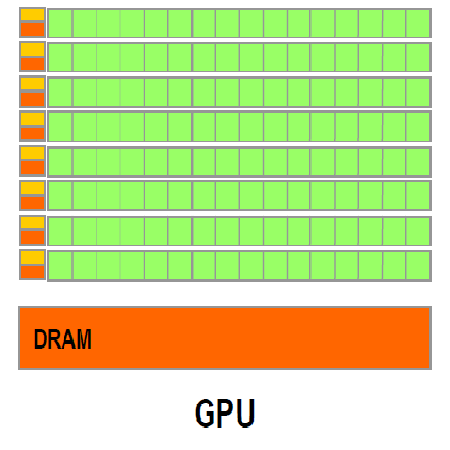
\includegraphics[width=0.9\textwidth]{Figs/GPU}\\
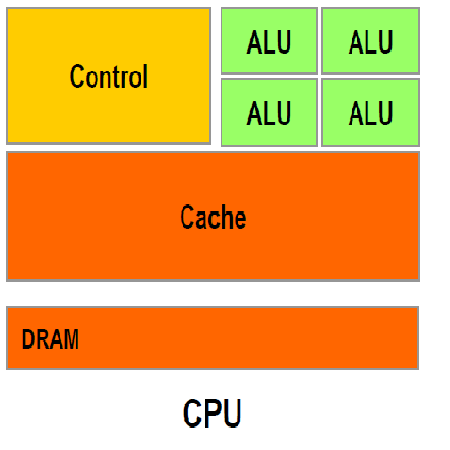
\includegraphics[width=0.9\textwidth]{Figs/CPU}\\
\end{center}
\end{column}
\end{columns}
}

%\subsection{Herramientas de programación }
\begin{frame}{Lenguajes de Descripción de Hardware}
\begin{columns}
	\column {0.5\textwidth}  
\begin{itemize}
\item Los lenguajes de descripción de hardware (HDL) permiten describir un circuitos digitales usando palabras y símbolos, y el software de desarrollo transforma esa descripciónen datos de configuración del FPGA para implementar la funcionalidad deseada.
\item Los lenguajes de descripción de hardware más populares son Verilog y VHDL. 
\item Permite el manejo de diferentes niveles de abstracción. 
\end{itemize}
\column {0.5\textwidth}  
\begin{center}
        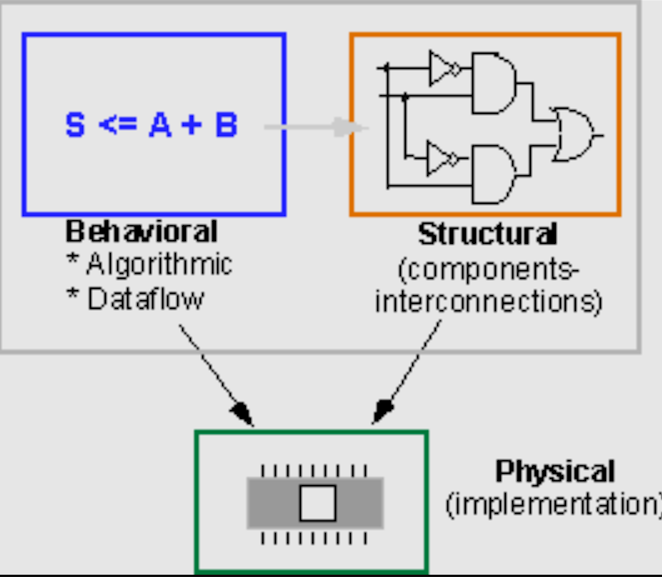
\includegraphics[width=0.6\textwidth]{Figs/NivelesAbstraccion}
\end{center}	
	  
\end{columns}
\end{frame}


\begin{frame}{VHDL}
\begin{columns}
	\column {0.5\textwidth}  
	
\begin{block}{VHDL}
\input{Lset_VHDL.tex}
			\lstinputlisting{01_CodigosFuente_Slides/Ejemplo.vhd}
\end{block}
	\column {0.5\textwidth}
	\begin{itemize}
\item VHDL es un lenguaje de especificación definido por el IEEE utilizado para describir circuitos digitales y automatizar el diseño electrónico. 
\item El acrónimo VHDL surge de dos acrónimos: VHSIC (Very High Speed Integrated Circuit) y HDL (Hardware Description Language).	
	\end{itemize}
        \begin{center}
        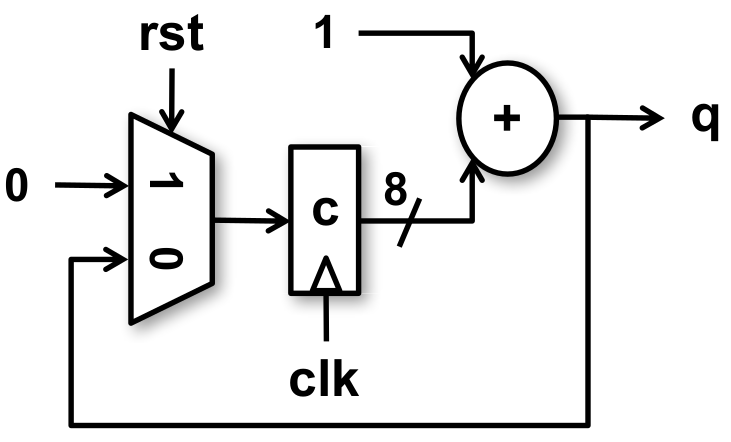
\includegraphics[width=0.6\textwidth]{Figs/Registro_8Bits}
        \end{center}	
	  
\end{columns}
\end{frame}

\begin{frame}{Verilog HDL}
\begin{columns}
	\column {0.5\textwidth}  
	\input{Lset_Verilog.tex}
\begin{block}{Verilog}
			\lstinputlisting{01_CodigosFuente_Slides/Prueba1.v}
\end{block}
	\column {0.5\textwidth} 
	\begin{itemize}
	\item Verilog HDL es un lenguaje de propósito general cuya sintaxis es parecida a lenguaje C.
    \item Es debilmente tipeado.
    \item Una versión mejorada es SystemVerilog con soporte de programación orientada a objetos (POO).
		\end{itemize}  
        \begin{center}
        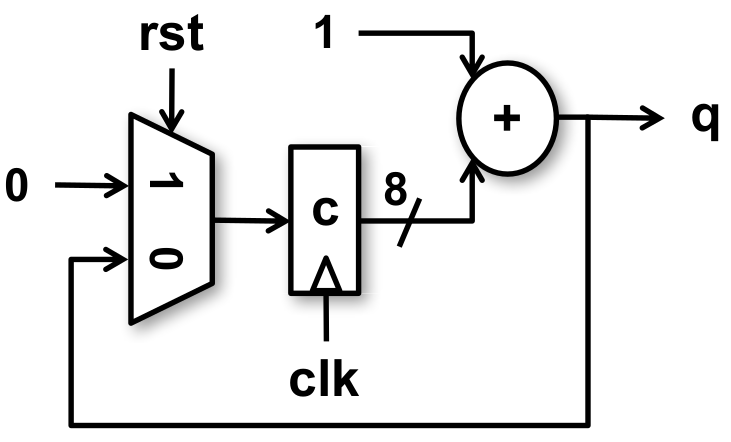
\includegraphics[width=0.6\textwidth]{Figs/Registro_8Bits}
        \end{center}	
	
\end{columns}
\end{frame}

\begin{frame}{High Level Synthesis (HLS)}
\begin{columns}
	\column {0.5\textwidth} 
    \begin{itemize}
        \item HLS es una tecnología que ayuda a transformar una descripción del comportamiento del hardware en un modelo RTL.	 
    \end{itemize}
\begin{block}{HLS}
\input{Lset_CPlusPlus.tex}
			\lstinputlisting{01_CodigosFuente_Slides/Codigo1.py}
\end{block}
	\column {0.5\textwidth}  
	\begin{itemize}
        \item El lenguaje de transferencia de registros (RTL) es una abstracción de diseño que modela un circuito digital síncrono en términos del flujo de señales digitales (datos) entre registros de hardware y las operaciones lógicas realizadas en esas señales.	
	\end{itemize}
        \begin{center}
        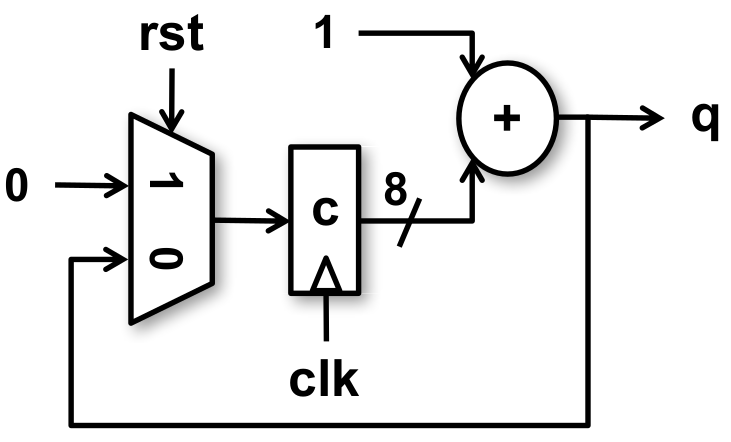
\includegraphics[width=0.6\textwidth]{Figs/Registro_8Bits}
        \end{center}		
\end{columns}
\end{frame}

